\documentclass[conference,a4paper]{IEEEtran}
\usepackage[T1]{fontenc}
\usepackage{cite,amsmath,amssymb,graphicx,booktabs,multirow,balance}
\usepackage[hidelinks]{hyperref}
\graphicspath{{figures/}}
\title{When Does Context Help Forecasting?\\An Empirical Study of Energy Systems}
\author{\IEEEauthorblockN{Xu Zheng\textsuperscript{1},
Jingchao Ni\textsuperscript{2}, Mo Sha\textsuperscript{1},
Dongsheng Luo\textsuperscript{3}}
\IEEEauthorblockA{\textsuperscript{1}Florida International University, Miami, FL, USA\\
\textsuperscript{2}University of Houston, Houston, TX, USA\\
\textsuperscript{3}Singapore Management University, Singapore\\
\{xzhen019,msha\}@fiu.edu, jni7@uh.edu, luodongsheng01@gmail.com}}
\begin{document}
\maketitle
\raggedbottom
\begin{abstract}
Energy systems produce operational records alongside power measurements:
storage states, charging limits, user requests, and indoor sensor readings.
These records can explain why devices with similar recent consumption follow
different future trajectories, but their forecasting value depends on both
the application and the predictor. We study this question across four public
source collections spanning water heaters, electric-vehicle charging, and
air conditioning. A shared evaluation task retains query-time information,
device identity, and the membership of the population being forecast.
Linear, tree, and neural references compare power history, device state, and
control information on matched cases. Storage records improve tree and neural
water-heater forecasts, while charging declarations improve group forecasts
beyond measured telemetry. Indoor measurements yield smaller and
model-dependent benefits. A second experiment reassigns operational records
within each query population and compares a fixed predictor with retraining
under the same reassignment. The substantial recovery on water heaters and
one charging site shows why sensitivity of a fitted model and the value of
correct record association must be evaluated separately. The study provides
source adapters, prepared tasks, and reproducible evaluation code for
context-aware energy forecasting.
\end{abstract}
\begin{IEEEkeywords}
time-series forecasting, energy systems, operational data, electric vehicles,
smart buildings, model evaluation
\end{IEEEkeywords}

\section{Introduction}
An energy-management system rarely observes only a load curve. A charging
station also records energy delivered, charging limits, and sometimes the
driver's requested energy and departure time. A water heater reports its
operating state and stored energy. A building controller links electricity
meters to room temperature and humidity. Collecting and maintaining these
records adds complexity, so a practical forecasting question is whether they
provide useful information beyond recent power consumption.

The answer matters for both model development and data integration. Two
vehicles drawing the same power may have very different remaining energy
requirements. Two idle heaters may resume operation at different times
because their storage states differ. In these settings, context can resolve
ambiguity in the power history. Conversely, a zone sensor shared by several
air conditioners may add little to a strong history-based predictor. The
presence of an intuitively relevant variable does not by itself establish
that a particular model can use it effectively.

The population being forecast is equally important. At a charging site,
forecasting demand from vehicles connected now is a different task from
forecasting the entire site's future demand, including arrivals. We focus
on the former: predict the power trajectories of devices identified at a
query time and, where supported, combine their forecasts into the demand of
that same group. This exposes a link between device information and aggregate
outcomes that disappears when every source is reduced to one load curve.

Energy-forecasting resources already cover rich covariates and several
aggregation levels. UrbanEV provides charging-demand data with spatial and
external information~\cite{li2025urbanev}; the Smarter Mobility Data Challenge
studies station, area, and overall occupancy~\cite{amaraouali2024occupancy}.
Device-level forecasting tools also support auxiliary information and
appliance behavior~\cite{neupane2016demand}. Our study complements these
resources by retaining the association between each operational record and
the device whose trajectory is predicted, together with the group to which
that device belongs.

We organize the evidence around two connected questions. First, when do
different kinds of context improve forecasts under fixed model recipes?
Second, when a predictor uses linked records, how much of its apparent
dependence on those links persists after retraining? The second question
requires more than removing inputs at inference. We compare correctly paired
records, reassigned records supplied to a fixed predictor, and a predictor
retrained on the same reassignment. Power histories and forecast targets are
unchanged throughout.

Across water heaters, two workplace charging sites, fast charging, and a
Bangkok office building, context yields distinct patterns. Device states help
tree and neural models on water heaters; driver declarations provide a
larger improvement in charging-group forecasts than the already measured
telemetry. Thermal context benefits a linear building-load model slightly
but does not improve its stronger tree reference. Retraining recovers much
of the reassignment loss in some settings, while another charging site shows
little recovery. These differences make the source, information condition,
and fitted recipe essential parts of the conclusion.

The contribution is an empirical study and a reusable evaluation task:
matched information comparisons across four attributed collections, a
record-association experiment connecting fixed-model sensitivity to
retraining, and source adapters that preserve the original device and group
semantics. The intended use is to guide choices about contextual inputs and
record integration in practical energy forecasting. Code, saved results,
and manuscript sources are available online.\footnote{\url{https://github.com/flyingdoog/context-energy-forecasting}}

\section{Related Work}
\subsection{Energy data and forecasting tasks}
ACN-Data links charging sessions to power, charging controls, and session
information~\cite{lee2019acndata}. EPFL's fast-charging release records two
charging plugs and heterogeneous vehicle sessions~\cite{desl2025level3},
while CU-BEMS couples circuit-level power to indoor environmental
measurements~\cite{pipattanasomporn2020cubems}. BPA's CTA-2045 demonstration
provides seasonal water-heater reports and control
records~\cite{bpa_cta2045}. These collections supply different operational
views of demand. We retain those differences within one prediction and
scoring interface, rather than treating seasons, charging sites, or building
floors as independent source collections.

The forecasting task also determines which metadata are usable. Requested
charging energy is information about future demand, whereas energy already
delivered describes the current state. A realized departure time is an
outcome unless it was declared earlier. Our input views distinguish these
fields at each query. This permits comparisons among history, state,
control, and declarations without changing the scored population.

\subsection{Models and record reliance}
We use a regularized linear reference, LightGBM~\cite{ke2017lightgbm}, and
N-HiTS~\cite{challu2023nhits} to examine how the value of context changes
across model families. The recipes remain fixed across information
conditions. The comparison therefore measures what these concrete
predictors obtain from the supplied records, rather than an optimal
achievable value of each information source.

Permutation-based analysis evaluates how a fitted predictor relies on
its inputs. Fisher \emph{et al.} distinguish reliance of one model from
reliance across well-performing models~\cite{fisher2019reliance}; conditional
approaches account for dependencies between retained and perturbed
features~\cite{molnar2024conditional}. Our intervention moves whole
auxiliary record blocks, including missingness masks, within the current
device group. Pairing evaluation-only reassignment with retraining makes
their different consequences visible in device-population forecasting.
It is a controlled use of these established ideas, not a new importance
estimator.

\section{Forecasting from Operational Records}
\subsection{Task and information available at a query}
At time $q$, let $G_q$ be the observed device population. For device $i$, let
$x_{iq}$ contain its power history and calendar features, and $z_{iq}$ contain
its available operational records and observation masks. A model returns
future mean powers
\begin{equation}
 \widehat{\boldsymbol y}_{iq}=f(x_{iq},z_{iq}), \qquad
 \widehat Y_{qj}=\sum_{i\in G_q}\widehat y_{iqj}.
 \label{eq:task}
\end{equation}
The second expression is the group-total forecast for bin $j$. Its target
uses the same membership $G_q$. Group-mean power divides both sides by
$|G_q|$. Device and group errors answer different questions because errors
can cancel or reinforce when summed.

\begin{figure}[t]
\centering
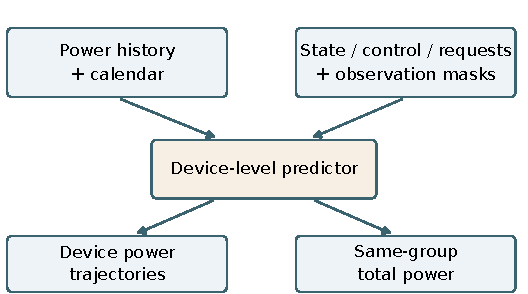
\includegraphics[width=\columnwidth]{task.pdf}
\caption{Context-aware forecasting for the devices observed at a query.
Information conditions change the auxiliary inputs, while the power
history, device population, and future scoring intervals remain fixed.}
\label{fig:task}
\end{figure}

We compare three primary information conditions: \emph{history},
\emph{history plus state}, and \emph{all telemetry}, the last additionally
including recorded controls. History includes the calendar. At Caltech, a
separate comparison adds query-available charging declarations to all
telemetry. For CU-BEMS, the state fields are observed temperature and
humidity; state and all telemetry coincide because control commands are
not supplied. Fig.~\ref{fig:task} shows the common task.

All inputs are restricted to information available by the query. Missing
records have explicit masks. A confirmed end of a charging session
establishes subsequent zero power for that session, but an unobserved tail
does not. Charging arrivals after the query are outside $G_q$. Where a
group member has an unsupported future target, the group is excluded from
complete-group scoring rather than silently reduced in size.

\subsection{Four source collections}
Table~\ref{tab:sources} summarizes the prepared evaluation populations.
BPA queries occur thirty minutes after a changed-command report, retaining
recent power and aligned previous-day/week profiles. Its synchronous groups
share the report time and command and contain at least ten label-eligible
devices. The measured outcome is reported power, which in this source is
partly estimated and calibrated. The groups represent supported observations
from the field study, not the entire utility fleet.

\begin{table*}[t]
\caption{Sources and evaluation support. Cases are device-query pairs, except
EPFL's one query per session; repeated queries are not independent devices.
The two ACN sites belong to one collection. Both later periods are retained.
CU-BEMS counts include all supported floors; Table II uses the matched thermal cohort.}
\label{tab:sources}
\centering\small
\setlength{\tabcolsep}{4pt}
\begin{tabular}{@{}llclrr@{}}
\toprule
Source / setting & Context beyond power & History & Later period & Cases & Dates\\
\midrule
\multirow{2}{*}{BPA heaters} & \multirow{2}{*}{Storage, flags, commands} & \multirow{2}{*}{24 h + profiles} & Spring 2018 &64,451&63\\
&&&Summer 2018&47,237&69\\
\multirow{2}{*}{ACN Caltech} & \multirow{2}{*}{State, pilot, declarations} & \multirow{2}{*}{60 min} & October 2019&4,858&31\\
&&&January 2020&3,983&30\\
\multirow{2}{*}{ACN Office} & \multirow{2}{*}{State, pilot} & \multirow{2}{*}{60 min} & October 2019&749&23\\
&&&January 2020&796&22\\
EPFL charging&SoC, energy, capacity, setpoint&First 10 min&March--July 2023&739&100\\
\multirow{2}{*}{CU-BEMS ACs} & \multirow{2}{*}{Zone temperature, humidity} & \multirow{2}{*}{60 min} & Sep.--Oct. 2019&154,316&61\\
&&&Nov.--Dec. 2019&135,839&61\\
\bottomrule
\end{tabular}
\end{table*}

ACN uses hourly queries for sessions already present at Caltech or Office.
Eligible groups contain at least two distinct charging stations and require
complete labels for their query-known cohort. The sites have different
information coverage: query-time declarations are observed at Caltech but
not in the selected Office records. EPFL contributes 1,771 eligible
fast-charging sessions on two plugs. Each query uses the first ten minutes
to predict actual delivered power; EPFL is evaluated at device level only.
Capacity estimates inferred from complete sessions and realized departures
are not inputs.

CU-BEMS contains 55 air-conditioning circuits in one Bangkok building, 51
with linked thermal sensor fields. The matched two-period comparison uses
44 circuits on Floors 2--5 and 7 and intersects dates across the compared
models. Floor 1 has no thermal fields; Floor 6's published file ends in
October. Their available data are retained in the package, but they do not
enter this matched thermal comparison. Several circuits can share a zone
sensor, so their context is different from a device-specific battery or
storage report.

\subsection{Splits, intervals, and error measures}
Splits follow time. BPA trains on 46,807 winter cases and validates on the
last fourteen observed winter dates, with targets crossing the boundary
excluded. ACN trains in April--June 2019 and validates in July. EPFL uses
2022 for training, January--February 2023 for validation, and March--July
for evaluation, yielding 946, 86, and 739 sessions. CU-BEMS trains in
April--June 2019 and validates in July--August. Table~\ref{tab:sources}
lists the later periods; no later period is used to tune the reference recipes.

BPA, ACN, and CU-BEMS score cumulative spans of 30, 90, and 150 minutes
using fifteen-minute target bins. EPFL scores 5, 15, and 30 minutes using
five-minute bins. Source timestamps and the distinction between point
reports and interval measurements are retained by the adapters. For a span
of $J$ bins, device MSE is the average of
$(\widehat y_{iqj}-y_{iqj})^2$ over its bins and eligible cases; MAE uses
absolute errors. Cases are averaged within each date, and dates then receive
equal weight. Span averages weight the three cumulative spans equally.

Power MSE and MAE are reported in kW$^2$ and kW, respectively. Group scores
use the same definitions after aggregation in~\eqref{eq:task}. CU-BEMS
additionally weights its common floors equally. We do not pool raw errors
across different power scales. Where intervals are quoted below, they are
the existing paired calendar-week bootstrap intervals from 1,500 draws,
conditional on the fitted predictors.

\section{Experiments}
\subsection{Reference models and comparison design}
Ridge uses an intercept, training-derived standardization, and a unit L2
penalty. LightGBM uses 100 trees, 31 leaves, and squared-error fitting for
each target bin. N-HiTS uses historical and current exogenous inputs,
known calendar features, and 1,000 squared-error training updates. Neural
results average the errors of three independently fitted seeds, not their
predictions. Each charging site or building floor is fitted separately.

The recipes are fixed, with no baseline hyperparameter search. Information
conditions share the same targets and eligible cases. The neural Caltech
declaration comparison keeps its input width fixed by replacing the added
fields with zeros in the telemetry-only control; CU-BEMS likewise zeroes
thermal slots in the history-only arm. These controls keep a change in
available information separate from a change in case selection or network
width.

\begin{table*}[t]
\caption{Device forecasting with different information conditions. MSE (kW$^2$) and MAE (kW) average the three native spans with equal date weights. CU-BEMS additionally weights its five common floors equally; its state and all-telemetry columns are the same thermal arm. Neural errors average three seeds. Bold marks the lowest error across information conditions within each model and row, including ties at displayed precision.}
\label{tab:device}
\centering\small
\setlength{\tabcolsep}{6pt}
\begin{tabular}{@{}llrrrrrr@{}}
\toprule
\multirow{2}{*}{Source / period} & \multirow{2}{*}{Model} & \multicolumn{2}{c}{History} & \multicolumn{2}{c}{History + state} & \multicolumn{2}{c}{All telemetry}\\
\cmidrule(lr){3-4}\cmidrule(lr){5-6}\cmidrule(l){7-8}
& & MSE & MAE & MSE & MAE & MSE & MAE\\
\midrule
\multirow{3}{*}{\shortstack[l]{BPA\\Spring}} & Ridge & \textbf{0.290} & \textbf{0.218} & 0.314 & 0.246 & 0.335 & 0.273 \\
 & LightGBM & 0.282 & 0.192 & 0.254 & 0.184 & \textbf{0.253} & \textbf{0.183} \\
 & N-HiTS & 0.322 & 0.208 & \textbf{0.297} & 0.191 & 0.298 & \textbf{0.189} \\
\addlinespace[2pt]
\multirow{3}{*}{\shortstack[l]{BPA\\Summer}} & Ridge & \textbf{0.239} & \textbf{0.198} & 0.256 & 0.223 & 0.334 & 0.290 \\
 & LightGBM & 0.228 & 0.176 & 0.197 & \textbf{0.166} & \textbf{0.196} & 0.167 \\
 & N-HiTS & 0.274 & 0.194 & \textbf{0.237} & \textbf{0.174} & 0.251 & 0.185 \\
\addlinespace[2pt]
\multirow{3}{*}{\shortstack[l]{Caltech\\Autumn}} & Ridge & \textbf{1.183} & \textbf{0.484} & 1.200 & 0.498 & 1.200 & 0.502 \\
 & LightGBM & 1.116 & 0.425 & 1.103 & 0.419 & \textbf{1.093} & \textbf{0.415} \\
 & N-HiTS & \textbf{1.202} & 0.455 & 1.207 & 0.440 & 1.208 & \textbf{0.437} \\
\addlinespace[2pt]
\multirow{3}{*}{\shortstack[l]{Caltech\\Winter}} & Ridge & \textbf{1.001} & \textbf{0.431} & 1.043 & 0.463 & 1.064 & 0.473 \\
 & LightGBM & 1.044 & 0.385 & 1.011 & 0.378 & \textbf{1.000} & \textbf{0.372} \\
 & N-HiTS & \textbf{1.075} & 0.406 & 1.080 & 0.396 & 1.081 & \textbf{0.392} \\
\addlinespace[2pt]
\multirow{3}{*}{\shortstack[l]{Office\\Autumn}} & Ridge & \textbf{2.221} & \textbf{0.856} & 2.588 & 0.946 & 2.788 & 0.997 \\
 & LightGBM & 2.819 & 0.893 & 2.689 & \textbf{0.886} & \textbf{2.665} & 0.889 \\
 & N-HiTS & 3.192 & \textbf{0.853} & \textbf{3.169} & 0.859 & 3.367 & 0.921 \\
\addlinespace[2pt]
\multirow{3}{*}{\shortstack[l]{Office\\Winter}} & Ridge & \textbf{2.623} & \textbf{0.937} & 2.916 & 0.992 & 2.965 & 1.023 \\
 & LightGBM & 3.231 & 1.042 & \textbf{2.923} & \textbf{0.995} & 2.942 & 1.004 \\
 & N-HiTS & 3.372 & \textbf{0.933} & \textbf{3.316} & 0.941 & 3.525 & 1.002 \\
\addlinespace[2pt]
\multirow{3}{*}{\shortstack[l]{EPFL\\Later}} & Ridge & 583.010 & 15.910 & \textbf{529.232} & \textbf{14.616} & 561.019 & 15.131 \\
 & LightGBM & 675.160 & 17.164 & 620.133 & 16.382 & \textbf{614.475} & \textbf{15.959} \\
 & N-HiTS & \textbf{740.517} & \textbf{17.457} & 798.949 & 18.326 & 874.857 & 18.772 \\
\addlinespace[2pt]
\multirow{3}{*}{\shortstack[l]{CU-BEMS\\Sep.--Oct.}} & Ridge & 13.784 & 1.491 & \textbf{13.630} & \textbf{1.460} & \textbf{13.630} & \textbf{1.460} \\
 & LightGBM & \textbf{3.015} & \textbf{0.427} & 3.317 & 0.473 & 3.317 & 0.473 \\
 & N-HiTS & \textbf{5.833} & \textbf{0.657} & 6.420 & 0.690 & 6.420 & 0.690 \\
\addlinespace[2pt]
\multirow{3}{*}{\shortstack[l]{CU-BEMS\\Nov.--Dec.}} & Ridge & 12.341 & 1.429 & \textbf{12.235} & \textbf{1.402} & \textbf{12.235} & \textbf{1.402} \\
 & LightGBM & \textbf{4.111} & \textbf{0.488} & 4.658 & 0.558 & 4.658 & 0.558 \\
 & N-HiTS & \textbf{6.871} & \textbf{0.698} & 7.662 & 0.763 & 7.662 & 0.763 \\
\bottomrule
\end{tabular}
\end{table*}


\begin{figure*}[t]
\centering
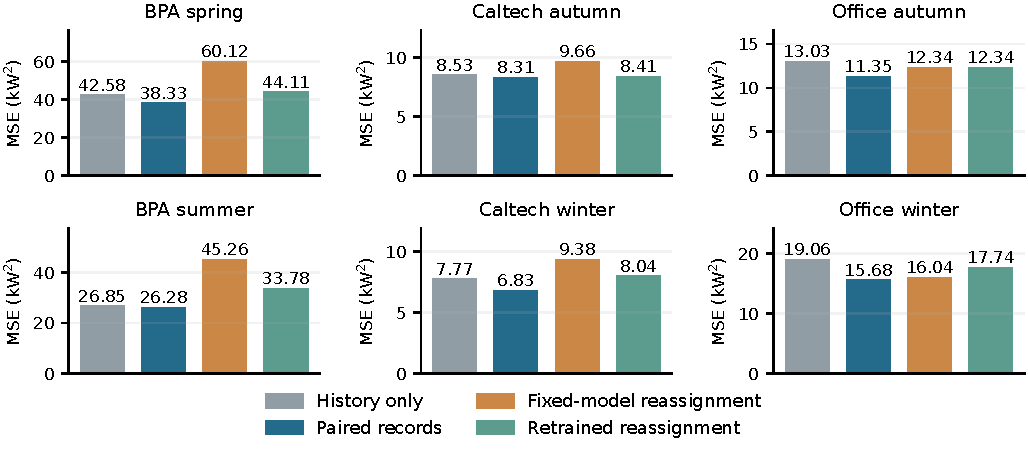
\includegraphics[width=.97\textwidth]{reassignment.pdf}
\caption{Group-total MSE for the four record-association arms, averaged over
native spans. Both reassigned arms use the same three within-query mappings.
Each panel has its own vertical scale. Retraining recovers much of the
fixed-model loss in BPA and Caltech, but not in Office.}
\label{fig:reassignment}
\end{figure*}

\subsection{Which contextual inputs help?}
Table~\ref{tab:device} reports device errors for all three fitted families,
every primary information condition, and both later periods where available.
The comparison shows that the benefit of context depends jointly on the
record type and the predictor.

\emph{Stored state helps nonlinear heater forecasts.}
On BPA, adding state lowers LightGBM MSE from 0.282 to 0.254 in spring
and from 0.228 to 0.197 in summer, with lower MAE in both periods.
N-HiTS follows the same pattern: 0.322 to 0.297 and 0.274 to 0.237.
Adding controls beyond state changes the tree results only slightly.
The linear reference does not share these gains. This pattern is consistent
with stored state being useful for predicting nonlinear operation, while
showing that additional fields alone do not determine the outcome.

\emph{Charging telemetry and user intent play different roles.}
State and control records improve the tree reference at both ACN sites.
At Caltech, however, measured telemetry does not substantially lower neural
MSE. Declarations provide a clearer improvement because requested energy
and intended departure describe demand that has not yet appeared in the
power trace. Table~\ref{tab:declarations} compares these inputs on the same
query-known groups. Adding declarations reduces span-average group-mean
MSE by approximately 19\% and 16\% for LightGBM in autumn and winter,
and by 25\% and 31\% for N-HiTS. MAE also decreases in all four comparisons.
Missing declarations remain masked; the comparison does not select only
sessions with complete user information.

\begin{table}[t]
\caption{Caltech group-mean forecasting with query-time demand declarations. MSE / MAE in kW$^2$ / kW; equal-span averages. The neural control has the same input width as the declaration arm.}
\label{tab:declarations}
\centering\small
\setlength{\tabcolsep}{3pt}
\begin{tabular}{@{}llll@{}}
\toprule
Model & Period & Telemetry & + declarations\\
& & MSE / MAE & MSE / MAE\\
\midrule
\multirow{2}{*}{LightGBM} & Autumn & 0.258 / 0.278 & 0.209 / 0.251 \\
 & Winter & 0.256 / 0.290 & 0.215 / 0.248 \\
\addlinespace[2pt]
\multirow{2}{*}{N-HiTS} & Autumn & 0.307 / 0.301 & 0.229 / 0.261 \\
 & Winter & 0.325 / 0.318 & 0.225 / 0.258 \\
\bottomrule
\end{tabular}
\end{table}


\emph{Fast charging and building sensors give different results.}
In EPFL, adding state lowers Ridge MSE from 583.010 to 529.232 and
LightGBM MSE from 675.160 to 620.133, with corresponding MAE improvements.
The neural reference worsens under the same information expansion. In
CU-BEMS, thermal inputs yield small gains for Ridge, while the stronger
history-based tree has lower errors without them in both later periods.
The records here are shared zone conditions, not individual stored-energy
states. The distinction is useful operationally: a strong history-only
reference provides a meaningful check before expanding the input pipeline.

Across these settings, model choice and information choice cannot be
separated. State helps the tree across the heater and charging collections,
but the neural gains depend on the particular fields and source. The
building example also shows why recording more covariates should be
accompanied by a matched information comparison, rather than presumed to
produce a better forecast.

\subsection{Correct associations, fixed-model sensitivity, and retraining}
The second experiment asks how context is used once it helps prediction.
Within a query group, we assign each receiving device an auxiliary record
from a deterministic within-group permutation $\pi_q$. Power history,
calendar, previous-day/week power profiles where available, and targets
stay with the receiving device. Auxiliary values and their masks move
together. Thus the group retains the same collection of operational
records, while individual associations change.

Four arms use the same fixed LightGBM recipe: history only, paired
records, a fitted paired predictor evaluated with reassigned records, and
a predictor retrained with reassigned records. Let their risks be
$R_H$, $R_P$, $R_F$, and $R_R$. Two useful differences are
\begin{equation}
 D_F=R_F-R_P,\qquad D_R=R_R-R_P.
\end{equation}
The first measures the fitted predictor's sensitivity; the second measures
the remaining gap under retraining with the chosen recipe. Their difference
$R_F-R_R$ is the recovered error. Three mapping seeds are used in both
reassigned arms, averaging errors across mappings. Constructing a mapping
does not read future labels. The experiment uses the ordinary telemetry
views, without the extra Caltech declarations.

Fig.~\ref{fig:reassignment} retains all six later site-period comparisons.
For BPA summer, group-total MSE rises from 26.277 with paired records to
45.256 when only evaluation records are reassigned. Retraining reduces it
to 33.780. Relative to the paired error, the fixed-model penalty is 72.23\%
(95\% interval 53.74--94.08\%), whereas the remaining retrained penalty is
28.55\% (23.86--35.08\%). Spring exhibits the same ordering. Correct
association is useful for this recipe, but the immediate failure of an
unchanged predictor is substantially larger than the gap after adaptation.

Caltech autumn illustrates an even stronger separation. Paired, fixed, and
retrained MSE are 8.313, 9.663, and 8.408. The fixed penalty is 16.24\%
(1.34--32.26\%), while the retrained penalty is 1.15\% (-5.86--9.69\%).
In winter, retraining again improves on the fixed arm but leaves a larger
gap: 6.827, 9.376, and 8.040, respectively. A fitted model's response to
reassignment therefore does not by itself determine how much performance
another fit can recover.

Office supplies a different result. In autumn, fixed and retrained MSE
are almost identical, 12.343 and 12.341; in winter, retraining increases
the error from 16.044 to 17.738. Both later periods still favor the paired
reference over history only. Consequently, useful context, fixed-model
sensitivity, and successful recovery are three separate empirical
properties, not interchangeable descriptions of one effect.

\section{Implications and Scope}
\subsection{Choosing inputs and maintaining records}
The first practical implication is to evaluate information conditions on
the same device population. Adding user requests can change which sessions
have complete inputs; dropping those with missing requests would also
change the forecasting problem. Explicit masks allow the input comparison
to retain the original cases. The Caltech experiment then attributes the
observed difference to the supplied declarations under its fixed recipes,
rather than to a different session subset.

Second, input types should be distinguished by their role. Stored energy,
energy already delivered, charging commands, and declared remaining demand
are not interchangeable measurements of ``state.'' The declaration results
show the value of representing future intent separately from observed
telemetry. The building results, in turn, caution against treating a shared
environmental measurement as if it were a device-specific state report.

Third, record-association checks should distinguish deployment sensitivity
from recovery after updating the predictor. A reassignment test on a fixed
model is relevant to an unexpected integration failure. Retraining asks a
different operational question: what accuracy does the same learning recipe
reach once trained with that representation? BPA and Caltech demonstrate
that the answers can differ substantially. Office demonstrates that
retraining is not automatically an effective remedy. Both measurements are
needed before converting a model's perturbation response into a claim
about the importance of a data linkage.

\subsection{Scope and reusable materials}
The evidence covers four collections and three device families, not all
energy applications. Seasonal periods and building floors probe different
operating conditions within their sources. The charging task concerns
devices observed at the query; total future site demand would require an
arrival model. EPFL's two-plug source supports session forecasting rather
than large-fleet conclusions. Results also condition on the fixed reference
recipes and available training data.

The reassignment intervention is synthetic. It preserves within-group
record contents but can alter their compatibility with retained histories;
it is not conditional resampling given every feature. The measured errors
describe predictor behavior under this specified intervention, not the
prevalence or causal cost of naturally occurring record errors. These
boundaries are particularly important when deciding whether retraining
can replace repairing an actual data pipeline.

The repository provides source adapters, a common submission/scoring
interface, reference code, and the saved scores used for every table and
figure. Preparation produces train/validation/evaluation packets with
observation masks and device/group identifiers; the evaluator keeps native
intervals and complete-group membership. Source acquisition instructions
and attribution accompany the code. Source records and prepared targets
are acquired locally under their providers' terms and are not redistributed
in the repository.

\balance
\section{Conclusion}
Operational context can improve energy forecasting, but its benefit depends
on what a record describes and how the predictor uses it. Stored state
helps nonlinear water-heater forecasts; charging declarations improve
group forecasts beyond telemetry; shared indoor measurements yield a
different, model-dependent pattern. Record reassignment further shows that
the sensitivity of a fitted predictor can greatly exceed the remaining
loss after retraining. Matched input comparisons and separate fixed-model
and retrained checks provide a practical way to evaluate these effects
while preserving the devices, groups, and future intervals of the
original forecasting task.

\section*{Acknowledgment}
OpenAI Codex assisted with study design, implementation, result analysis,
and drafting and editing the abstract and Sections I--VI, including table
and figure code. Anthropic Claude assisted with manuscript review.
The numerical results derive from the attributed source records and
completed experiments; no source observations were generated by these tools.

\bibliographystyle{IEEEtran}
\bibliography{references}
\end{document}
